\documentclass[tikz,border=2pt]{standalone}
\usepackage{amsmath,amssymb}
\usetikzlibrary{arrows.meta,calc,decorations.pathmorphing,positioning,shapes.geometric}

\definecolor{qblue}{HTML}{0072B2}
\definecolor{qbluefill}{HTML}{DCEEF7}
\definecolor{qverm}{HTML}{D55E00}
\definecolor{qgold}{HTML}{B97800}
\definecolor{qink}{HTML}{1B1F23}
\definecolor{qmuted}{HTML}{5E6670}
\definecolor{qgrid}{HTML}{D8DEE5}

\tikzset{
  waveblue/.style={qblue,line width=.75pt,decorate,
    decoration={snake,amplitude=.24mm,segment length=1.55mm}},
  wavegold/.style={qgold,line width=.75pt,decorate,
    decoration={snake,amplitude=.24mm,segment length=1.55mm}},
  exchange/.style={qverm,line width=1.35pt},
  vertex/.style={diamond,draw=qverm,fill=white,inner sep=1.35pt,line width=.8pt},
  freebox/.style={rounded corners=.6mm,draw=qblue,fill=qbluefill,
    minimum width=1.55cm,minimum height=.82cm,line width=.8pt},
  head/.style={font=\sffamily\bfseries\footnotesize,text=qink},
  panel/.style={font=\sffamily\bfseries\scriptsize,text=qink},
  small/.style={font=\sffamily\scriptsize,text=qink},
  muted/.style={font=\sffamily\scriptsize,text=qmuted},
}

\begin{document}
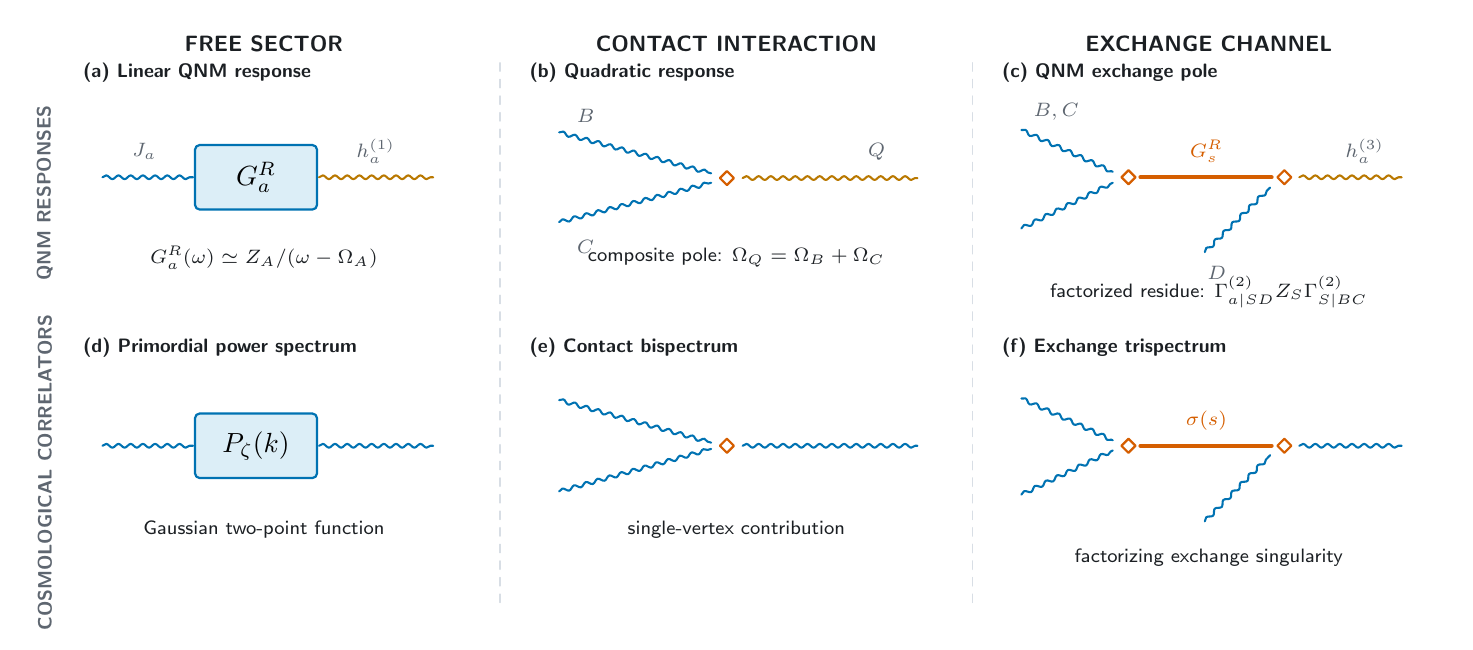
\begin{tikzpicture}[x=1cm,y=1cm,line cap=round,line join=round,>=Latex]
  \useasboundingbox (0,0) rectangle (18,7.55);
  \draw[qgrid,dashed,line width=.55pt] (6.0,.25)--(6.0,7.15);
  \draw[qgrid,dashed,line width=.55pt] (12.0,.25)--(12.0,7.15);

  \node[head] at (3.0,7.34) {FREE SECTOR};
  \node[head] at (9.0,7.34) {CONTACT INTERACTION};
  \node[head] at (15.0,7.34) {EXCHANGE CHANNEL};
  \node[font=\sffamily\bfseries\scriptsize,text=qmuted,rotate=90]
    at (.22,5.45) {QNM RESPONSES};
  \node[font=\sffamily\bfseries\scriptsize,text=qmuted,rotate=90]
    at (.22,1.90) {COSMOLOGICAL CORRELATORS};

  % (a) Linear QNM response.
  \node[panel,anchor=west] at (.58,6.98) {(a) Linear QNM response};
  \draw[waveblue] (.95,5.65)--(2.10,5.65);
  \node[freebox] (gr) at (2.90,5.65) {$G_a^R$};
  \draw[wavegold] (3.70,5.65)--(5.15,5.65);
  \node[muted] at (1.48,5.98) {$J_a$};
  \node[muted] at (4.42,5.98) {$h_a^{(1)}$};
  \node[small] at (3.0,4.63) {$G_a^R(\omega)\simeq Z_A/(\omega-\Omega_A)$};

  % (b) Quadratic contact.
  \node[panel,anchor=west] at (6.25,6.98) {(b) Quadratic response};
  \draw[waveblue] (6.75,6.22)--(8.68,5.70);
  \draw[waveblue] (6.75,5.08)--(8.68,5.58);
  \node[vertex] (v2) at (8.88,5.64) {};
  \draw[wavegold] (9.08,5.64)--(11.30,5.64);
  \node[muted,anchor=west] at (6.85,6.43) {$B$};
  \node[muted,anchor=west] at (6.85,4.76) {$C$};
  \node[muted] at (10.78,5.98) {$Q$};
  \node[small] at (9.0,4.63) {composite pole: $\Omega_Q=\Omega_B+\Omega_C$};

  % (c) Exchanged QNM.
  \node[panel,anchor=west] at (12.25,6.98) {(c) QNM exchange pole};
  \draw[waveblue] (12.62,6.25)--(13.78,5.72);
  \draw[waveblue] (12.62,5.00)--(13.78,5.58);
  \node[vertex] (vs) at (13.98,5.65) {};
  \draw[exchange] (14.13,5.65)--(15.80,5.65);
  \node[vertex] (va) at (15.96,5.65) {};
  \draw[waveblue] (14.95,4.70)--(15.78,5.52);
  \draw[wavegold] (16.15,5.65)--(17.45,5.65);
  \node[font=\sffamily\scriptsize\bfseries,text=qverm] at (14.97,5.98) {$G_s^R$};
  \node[muted,anchor=west] at (12.65,6.48) {$B,C$};
  \node[muted] at (15.10,4.43) {$D$};
  \node[muted] at (16.98,5.98) {$h_a^{(3)}$};
  \node[small] at (15.0,4.19)
    {factorized residue: $\Gamma^{(2)}_{a|SD}Z_S\Gamma^{(2)}_{S|BC}$};

  % (d) Gaussian two-point data.
  \node[panel,anchor=west] at (.58,3.48) {(d) Primordial power spectrum};
  \draw[waveblue] (.95,2.24)--(2.10,2.24);
  \node[freebox] (pz) at (2.90,2.24) {$P_\zeta(k)$};
  \draw[waveblue] (3.70,2.24)--(5.15,2.24);
  \node[small] at (3.0,1.18) {Gaussian two-point function};

  % (e) Contact non-Gaussianity.
  \node[panel,anchor=west] at (6.25,3.48) {(e) Contact bispectrum};
  \draw[waveblue] (6.75,2.82)--(8.68,2.28);
  \draw[waveblue] (6.75,1.66)--(8.68,2.20);
  \node[vertex] at (8.88,2.24) {};
  \draw[waveblue] (9.08,2.24)--(11.30,2.24);
  \node[small] at (9.0,1.18) {single-vertex contribution};

  % (f) Particle exchange.
  \node[panel,anchor=west] at (12.25,3.48) {(f) Exchange trispectrum};
  \draw[waveblue] (12.62,2.84)--(13.78,2.31);
  \draw[waveblue] (12.62,1.62)--(13.78,2.18);
  \node[vertex] at (13.98,2.24) {};
  \draw[exchange] (14.13,2.24)--(15.80,2.24);
  \node[vertex] at (15.96,2.24) {};
  \draw[waveblue] (14.95,1.28)--(15.78,2.12);
  \draw[waveblue] (16.15,2.24)--(17.45,2.24);
  \node[font=\sffamily\scriptsize\bfseries,text=qverm] at (14.97,2.56) {$\sigma(s)$};
  \node[small] at (15.0,.82) {factorizing exchange singularity};
\end{tikzpicture}
\end{document}
